\section{Thực nghiệm, đánh giá}
\label{sec:TNDG}
\subsection{Dữ liệu thực nghiệm}
\label{subsec:DLTN}

\subsection{Công cụ dùng trong thực nghiệm}
\label{subsec:tools}
\begin{frame}{Thực nghiệm, đánh giá}
\begin{block}{\ref{subsec:DLTN}. Dữ liệu thực nghiệm}
	\begin{itemize}
		\item Dữ liệu của trò chơi Code Hunt
		\item Dữ liệu do tôi tự xây dựng.
	\end{itemize}
\end{block}
\begin{block}{\ref{subsec:tools}. Công cụ dùng trong thực nghiệm}
\begin{itemize}
\item Microsoft Visual Studio
\item Công cụ sinh dữ liệu thử PEX
\end{itemize}
\end{block}
\end{frame}

\subsection{Kết quả thực nghiệm}
\label{subsec:DGKQTN}
\begin{frame}{Thực nghiệm, đánh giá}
\begin{block}{\ref{subsec:DGKQTN}. Kết quả thực nghiệm}
\centering
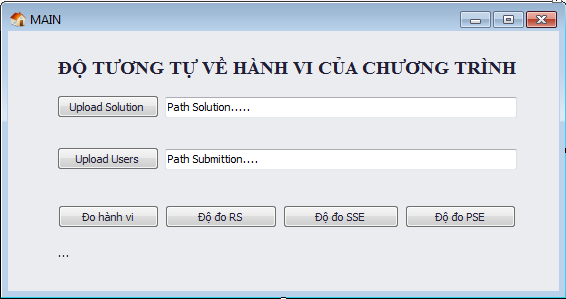
\includegraphics[width=0.8\linewidth]{images/main.png}
\begin{itemize}
	\item Hai nút Upload Solution và Upload Users cho phép tải 
	chương trình tham chiếu và chương trình cần tính
	\item Bên dưới là các nút đo độ tương tự hành vi của chương
	trình, và kết quả các phép đo RS, SSE và PSE.
\end{itemize}	
\end{block}
\end{frame}

\begin{frame}{Thực nghiệm, đánh giá}
\begin{block}{\ref{subsec:DGKQTN}. Kết quả thực nghiệm}
	\centering
	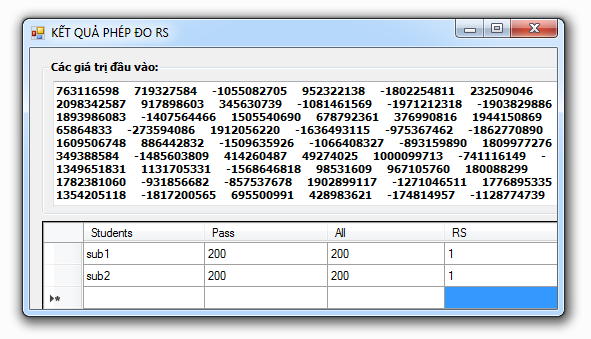
\includegraphics[width=0.6\linewidth]{images/kq_rs.png} \\	
	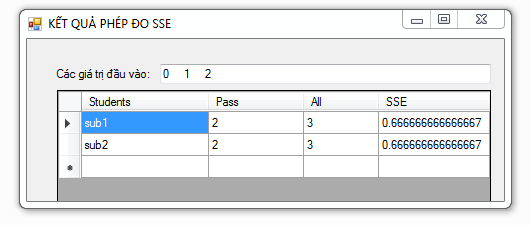
\includegraphics[width=0.6\linewidth]{images/kq_sse.png} \\
	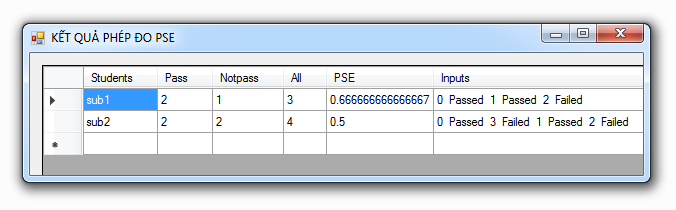
\includegraphics[width=0.6\linewidth]{images/kq_pse.png}	
\end{block}
\end{frame}

\begin{frame}{Thực nghiệm, đánh giá}
\begin{block}{\ref{subsec:DGKQTN}. Kết quả thực nghiệm}
\begin{itemize}
	\item Phép đo RS
	\begin{itemize}
		\item Ưu điểm: Đánh giá khách quan, tốc độ xử lý nhanh, 
		ít tốn tài nguyên máy tính
		\item Hạn chế: Không quan tâm đến hành vi của chương 
		trình, chỉ quan tâm đến dữ liệu vào và ra của chương trình
	\end{itemize} \pause
	\item Phép đo SSE
	\begin{itemize}
		\item Ưu điểm: Sử dụng kỹ thuật DSE để sinh ra tập các 
		giá trị đầu vào của chương trình, phép đo PSE cho kết quả 
		chính xác hơn phép đo RS
		\item Hạn chế: Không quan tâm đến chương trình cần phân tích, 
		tốn tài nguyên máy tính, thời gian thực thi chậm hơn phép đo RS
	\end{itemize} \pause
	\item Phép đo PSE
	\begin{itemize}
		\item Ưu điểm: Tập giá trị đầu vào của chương trình có độ phủ cao, 
		kết quả độ tương tự hành vi của chương trình theo phép đo PSE tốt hơn phép đo SSE
		\item Hạn chế: Tốn tài nguyên máy tính và thời 
		gian thực thi lâu hơn phép đo SSE
	\end{itemize}
\end{itemize}
\end{block}
\end{frame}

\subsection{Hướng phát triển và khả năng ứng dụng}
\label{subsec:HPTKNUD}
\subsubsection*{Hướng phát triển}
\label{subsubsec:HPT}
\subsubsection*{Khả năng ứng dụng}
\label{subsubsec:KNUD}
\begin{frame}{Hướng phát triển và khả năng ứng dụng}
	\begin{block}{\ref{subsubsec:HPT}. Hướng phát triển}
		\begin{itemize}
			\item Cải tiến các phép đo để kết quả được chính xác hơn
			\item Tích hợp thêm một số ngôn ngữ Java, C++...
		\end{itemize}
	\end{block} \pause
	\begin{block}{\ref{subsubsec:KNUD}. Khả năng ứng dụng}
		\begin{itemize}
			\item Đánh giá tiến bộ trong lập trình
			\item Xếp hạng tự động
			\item Gợi ý giải pháp lập trình
		\end{itemize}
	\end{block}
\end{frame}

\begin{frame}{KẾT THÚC}
\centering
{\Huge XIN CẢM ƠN!}
\end{frame}

